% Options for packages loaded elsewhere
\PassOptionsToPackage{unicode}{hyperref}
\PassOptionsToPackage{hyphens}{url}
\PassOptionsToPackage{dvipsnames,svgnames,x11names}{xcolor}
%
\documentclass[
]{article}
\title{Module 7: Recommended Exercises}
\usepackage{etoolbox}
\makeatletter
\providecommand{\subtitle}[1]{% add subtitle to \maketitle
  \apptocmd{\@title}{\par {\large #1 \par}}{}{}
}
\makeatother
\subtitle{TMA4268 Statistical Learning V2022}
\author{Emma Skarstein, Daesoo Lee, Stefanie Muff \and Department of
Mathematical Sciences, NTNU}
\date{Feb 28, 2022}

\usepackage{amsmath,amssymb}
\usepackage{lmodern}
\usepackage{iftex}
\ifPDFTeX
  \usepackage[T1]{fontenc}
  \usepackage[utf8]{inputenc}
  \usepackage{textcomp} % provide euro and other symbols
\else % if luatex or xetex
  \usepackage{unicode-math}
  \defaultfontfeatures{Scale=MatchLowercase}
  \defaultfontfeatures[\rmfamily]{Ligatures=TeX,Scale=1}
\fi
% Use upquote if available, for straight quotes in verbatim environments
\IfFileExists{upquote.sty}{\usepackage{upquote}}{}
\IfFileExists{microtype.sty}{% use microtype if available
  \usepackage[]{microtype}
  \UseMicrotypeSet[protrusion]{basicmath} % disable protrusion for tt fonts
}{}
\makeatletter
\@ifundefined{KOMAClassName}{% if non-KOMA class
  \IfFileExists{parskip.sty}{%
    \usepackage{parskip}
  }{% else
    \setlength{\parindent}{0pt}
    \setlength{\parskip}{6pt plus 2pt minus 1pt}}
}{% if KOMA class
  \KOMAoptions{parskip=half}}
\makeatother
\usepackage{xcolor}
\IfFileExists{xurl.sty}{\usepackage{xurl}}{} % add URL line breaks if available
\IfFileExists{bookmark.sty}{\usepackage{bookmark}}{\usepackage{hyperref}}
\hypersetup{
  pdftitle={Module 7: Recommended Exercises},
  pdfauthor={Emma Skarstein, Daesoo Lee, Stefanie Muff; Department of Mathematical Sciences, NTNU},
  colorlinks=true,
  linkcolor={Maroon},
  filecolor={Maroon},
  citecolor={Blue},
  urlcolor={blue},
  pdfcreator={LaTeX via pandoc}}
\urlstyle{same} % disable monospaced font for URLs
\usepackage[margin=1in]{geometry}
\usepackage{color}
\usepackage{fancyvrb}
\newcommand{\VerbBar}{|}
\newcommand{\VERB}{\Verb[commandchars=\\\{\}]}
\DefineVerbatimEnvironment{Highlighting}{Verbatim}{commandchars=\\\{\}}
% Add ',fontsize=\small' for more characters per line
\usepackage{framed}
\definecolor{shadecolor}{RGB}{248,248,248}
\newenvironment{Shaded}{\begin{snugshade}}{\end{snugshade}}
\newcommand{\AlertTok}[1]{\textcolor[rgb]{0.94,0.16,0.16}{#1}}
\newcommand{\AnnotationTok}[1]{\textcolor[rgb]{0.56,0.35,0.01}{\textbf{\textit{#1}}}}
\newcommand{\AttributeTok}[1]{\textcolor[rgb]{0.77,0.63,0.00}{#1}}
\newcommand{\BaseNTok}[1]{\textcolor[rgb]{0.00,0.00,0.81}{#1}}
\newcommand{\BuiltInTok}[1]{#1}
\newcommand{\CharTok}[1]{\textcolor[rgb]{0.31,0.60,0.02}{#1}}
\newcommand{\CommentTok}[1]{\textcolor[rgb]{0.56,0.35,0.01}{\textit{#1}}}
\newcommand{\CommentVarTok}[1]{\textcolor[rgb]{0.56,0.35,0.01}{\textbf{\textit{#1}}}}
\newcommand{\ConstantTok}[1]{\textcolor[rgb]{0.00,0.00,0.00}{#1}}
\newcommand{\ControlFlowTok}[1]{\textcolor[rgb]{0.13,0.29,0.53}{\textbf{#1}}}
\newcommand{\DataTypeTok}[1]{\textcolor[rgb]{0.13,0.29,0.53}{#1}}
\newcommand{\DecValTok}[1]{\textcolor[rgb]{0.00,0.00,0.81}{#1}}
\newcommand{\DocumentationTok}[1]{\textcolor[rgb]{0.56,0.35,0.01}{\textbf{\textit{#1}}}}
\newcommand{\ErrorTok}[1]{\textcolor[rgb]{0.64,0.00,0.00}{\textbf{#1}}}
\newcommand{\ExtensionTok}[1]{#1}
\newcommand{\FloatTok}[1]{\textcolor[rgb]{0.00,0.00,0.81}{#1}}
\newcommand{\FunctionTok}[1]{\textcolor[rgb]{0.00,0.00,0.00}{#1}}
\newcommand{\ImportTok}[1]{#1}
\newcommand{\InformationTok}[1]{\textcolor[rgb]{0.56,0.35,0.01}{\textbf{\textit{#1}}}}
\newcommand{\KeywordTok}[1]{\textcolor[rgb]{0.13,0.29,0.53}{\textbf{#1}}}
\newcommand{\NormalTok}[1]{#1}
\newcommand{\OperatorTok}[1]{\textcolor[rgb]{0.81,0.36,0.00}{\textbf{#1}}}
\newcommand{\OtherTok}[1]{\textcolor[rgb]{0.56,0.35,0.01}{#1}}
\newcommand{\PreprocessorTok}[1]{\textcolor[rgb]{0.56,0.35,0.01}{\textit{#1}}}
\newcommand{\RegionMarkerTok}[1]{#1}
\newcommand{\SpecialCharTok}[1]{\textcolor[rgb]{0.00,0.00,0.00}{#1}}
\newcommand{\SpecialStringTok}[1]{\textcolor[rgb]{0.31,0.60,0.02}{#1}}
\newcommand{\StringTok}[1]{\textcolor[rgb]{0.31,0.60,0.02}{#1}}
\newcommand{\VariableTok}[1]{\textcolor[rgb]{0.00,0.00,0.00}{#1}}
\newcommand{\VerbatimStringTok}[1]{\textcolor[rgb]{0.31,0.60,0.02}{#1}}
\newcommand{\WarningTok}[1]{\textcolor[rgb]{0.56,0.35,0.01}{\textbf{\textit{#1}}}}
\usepackage{graphicx}
\makeatletter
\def\maxwidth{\ifdim\Gin@nat@width>\linewidth\linewidth\else\Gin@nat@width\fi}
\def\maxheight{\ifdim\Gin@nat@height>\textheight\textheight\else\Gin@nat@height\fi}
\makeatother
% Scale images if necessary, so that they will not overflow the page
% margins by default, and it is still possible to overwrite the defaults
% using explicit options in \includegraphics[width, height, ...]{}
\setkeys{Gin}{width=\maxwidth,height=\maxheight,keepaspectratio}
% Set default figure placement to htbp
\makeatletter
\def\fps@figure{htbp}
\makeatother
\setlength{\emergencystretch}{3em} % prevent overfull lines
\providecommand{\tightlist}{%
  \setlength{\itemsep}{0pt}\setlength{\parskip}{0pt}}
\setcounter{secnumdepth}{-\maxdimen} % remove section numbering
\ifLuaTeX
  \usepackage{selnolig}  % disable illegal ligatures
\fi

\begin{document}
\maketitle

The original version of this exercise sheet was developed in 2019 by
Andreas Strand and colleagues. Thanks for the permission to build on it.

\hypertarget{problem-1}{%
\subsection{Problem 1}\label{problem-1}}

Let us take a look at the \texttt{Auto} data set. We want to model miles
per gallon \texttt{mpg} by engine horsepower \texttt{horsepower}.
Separate the observations into training and test. A training set is
plotted below.

Perform polynomial regression of degree 1, 2, 3 and 4. Use
\texttt{lines()} to add the fitted values to the plot below.

Also plot the test error depending on polynomial degree.

\begin{Shaded}
\begin{Highlighting}[]
\FunctionTok{library}\NormalTok{(ISLR)}
\CommentTok{\# extract only the two variables from Auto}
\NormalTok{ds }\OtherTok{=}\NormalTok{ Auto[}\FunctionTok{c}\NormalTok{(}\StringTok{"horsepower"}\NormalTok{,}\StringTok{"mpg"}\NormalTok{)]}
\NormalTok{n }\OtherTok{=} \FunctionTok{nrow}\NormalTok{(ds)}
\CommentTok{\#which degrees we will look at}
\NormalTok{deg }\OtherTok{=} \DecValTok{1}\SpecialCharTok{:}\DecValTok{4}
\FunctionTok{set.seed}\NormalTok{(}\DecValTok{1}\NormalTok{)}
\CommentTok{\#training ids for training set}
\NormalTok{tr }\OtherTok{=} \FunctionTok{sample.int}\NormalTok{(n, n}\SpecialCharTok{/}\DecValTok{2}\NormalTok{)}
\CommentTok{\# plot of training data}
\FunctionTok{plot}\NormalTok{(ds[tr,], }\AttributeTok{col =} \StringTok{"darkgrey"}\NormalTok{, }\AttributeTok{main =} \StringTok{"Polynomial regression"}\NormalTok{)}
\end{Highlighting}
\end{Shaded}

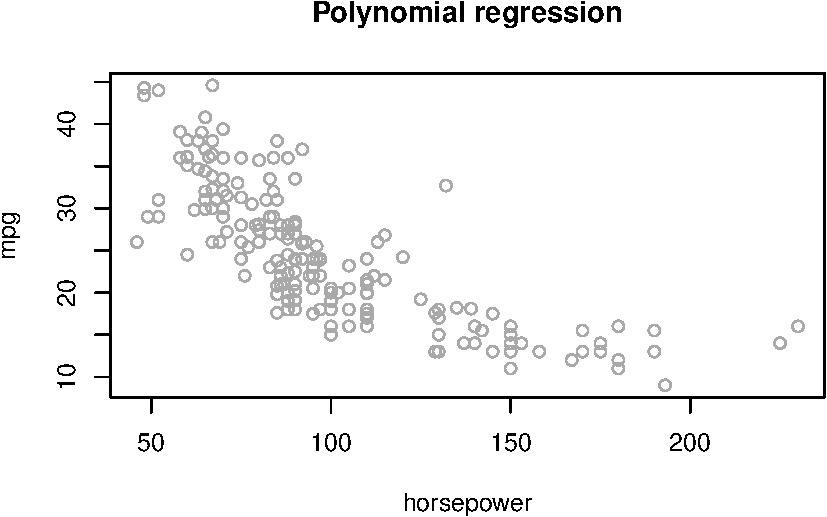
\includegraphics{RecEx7_files/figure-latex/unnamed-chunk-1-1.pdf}

\hypertarget{problem-2}{%
\subsection{Problem 2}\label{problem-2}}

We will continue working with the \texttt{Auto} data set. The variable
\texttt{origin} is 1,2 or 3, corresponding to American, European or
Japanese origin. Use \texttt{factor(origin)} for conversion to a factor
variable. Predict \texttt{mpg} by origin with a linear model. Plot the
fitted values and approximative 95 percent confidence intervals.
Selecting \texttt{se\ =\ T} in \texttt{predict()} gives standard errors
of the prediction.

\begin{itemize}
\item
  Hint: make a new dataframe of the three origins (as factors) and use
  this new data in your predict function.
\item
  Hint: to plot the confidence intervals, you can add
  \texttt{geom\_segment(aes(x=origin,\ y=lwr,\ xend\ =\ origin,\ yend=upr))}
  to your ggplot, where \texttt{origin}, \texttt{lwr} and \texttt{upr}
  comes from a dataframe with \texttt{lwr} as the lower bound and
  \texttt{upr} as the upper bound.
\end{itemize}

\hypertarget{problem-3}{%
\subsection{Problem 3}\label{problem-3}}

Now, let us look at the \texttt{Wage} data set. The section on Additive
Models
\href{https://github.com/stefaniemuff/statlearning/blob/master/7BeyondLinear/7slides.pdf}{(slides
28-34 in the pdf)} explains how we can create an AM by adding components
together. One component we saw is a natural spline in \texttt{year} with
one knot. Derive the expression for the design matrix \(\mathbf X_2\)
from the natural spline basis: \[
b_1(x_i) = x_i, \quad b_{k+2}(x_i) = d_k(x_i)-d_K(x_i),\; k = 0, \ldots, K - 1,\\
\] \[
d_k(x_i) = \frac{(x_i-c_k)^3_+-(x_i-c_{K+1})^3_+}{c_{K+1}-c_k}.
\]

\hypertarget{problem-4}{%
\subsection{Problem 4}\label{problem-4}}

We will continue working with the same AM as in problem 3. The R call
\texttt{model.matrix(\textasciitilde{}\ bs(age,knots=c(40,60))\ +\ ns(year,knots=2006)\ +\ education)}
gives a design matrix for the AM. This matrix is what \texttt{gam()}
uses. However, it does not equal our design matrix for AM
\(\mathbf X = (\mathbf{1}, \mathbf{X}_1, \mathbf{X}_2, \mathbf{X}_3)\).
The predicted responses will still be the same.

Write code that produces \(\mathbf X\). The code below may be useful.

\begin{Shaded}
\begin{Highlighting}[]
\CommentTok{\#X\_1}
\NormalTok{mybs }\OtherTok{=} \ControlFlowTok{function}\NormalTok{(x,knots)\{}
  \FunctionTok{cbind}\NormalTok{(x,x}\SpecialCharTok{\^{}}\DecValTok{2}\NormalTok{,x}\SpecialCharTok{\^{}}\DecValTok{3}\NormalTok{,}\FunctionTok{sapply}\NormalTok{(knots,}\ControlFlowTok{function}\NormalTok{(y) }\FunctionTok{pmax}\NormalTok{(}\DecValTok{0}\NormalTok{,x}\SpecialCharTok{{-}}\NormalTok{y)}\SpecialCharTok{\^{}}\DecValTok{3}\NormalTok{))}
\NormalTok{\}}

\NormalTok{d }\OtherTok{=} \ControlFlowTok{function}\NormalTok{(c, cK, x) (}\FunctionTok{pmax}\NormalTok{(}\DecValTok{0}\NormalTok{,x}\SpecialCharTok{{-}}\NormalTok{c)}\SpecialCharTok{\^{}}\DecValTok{3}\SpecialCharTok{{-}}\FunctionTok{pmax}\NormalTok{(}\DecValTok{0}\NormalTok{,x}\SpecialCharTok{{-}}\NormalTok{cK)}\SpecialCharTok{\^{}}\DecValTok{3}\NormalTok{)}\SpecialCharTok{/}\NormalTok{(cK}\SpecialCharTok{{-}}\NormalTok{c)}
\CommentTok{\#X\_2}
\NormalTok{myns }\OtherTok{=} \ControlFlowTok{function}\NormalTok{(x,knots)\{}
\NormalTok{  kn }\OtherTok{=} \FunctionTok{c}\NormalTok{(}\FunctionTok{min}\NormalTok{(x), knots, }\FunctionTok{max}\NormalTok{(x))}
\NormalTok{  K }\OtherTok{=} \FunctionTok{length}\NormalTok{(kn)}
\NormalTok{  sub }\OtherTok{=} \FunctionTok{d}\NormalTok{(kn[K}\DecValTok{{-}1}\NormalTok{],kn[K],x)}
  \FunctionTok{cbind}\NormalTok{(x,}\FunctionTok{sapply}\NormalTok{(kn[}\DecValTok{1}\SpecialCharTok{:}\NormalTok{(K}\DecValTok{{-}2}\NormalTok{)],d,kn[K],x)}\SpecialCharTok{{-}}\NormalTok{sub)}
\NormalTok{\}}
\CommentTok{\#X\_3}
\NormalTok{myfactor }\OtherTok{=} \ControlFlowTok{function}\NormalTok{(x) }\FunctionTok{model.matrix}\NormalTok{(}\SpecialCharTok{\textasciitilde{}}\NormalTok{x)[,}\SpecialCharTok{{-}}\DecValTok{1}\NormalTok{]}
\end{Highlighting}
\end{Shaded}

If the code is valid, the predicted response
\(\hat{\mathbf y} = \mathbf X(\mathbf X^\mathsf{T} \mathbf X)^{-1} \mathbf X^\mathsf{T} \mathbf y\)
should be the same as when using the built-in R function \texttt{gam()}.

\textbf{R-hints}:

\begin{Shaded}
\begin{Highlighting}[]
\CommentTok{\#install.packages("gam"")}
\FunctionTok{library}\NormalTok{(gam)}
\FunctionTok{library}\NormalTok{(ISLR)}
\CommentTok{\# Figure out how to define your X{-}matrix (this is perhaps a bit tricky!)}
\NormalTok{X }\OtherTok{=}\NormalTok{ ...}
\CommentTok{\# fitted model with our X}
\NormalTok{myhat }\OtherTok{=} \FunctionTok{lm}\NormalTok{(wage }\SpecialCharTok{\textasciitilde{}}\NormalTok{ X }\SpecialCharTok{{-}} \DecValTok{1}\NormalTok{)}\SpecialCharTok{$}\NormalTok{fit}
\CommentTok{\# fitted model with gam}
\NormalTok{yhat }\OtherTok{=} \FunctionTok{gam}\NormalTok{(wage }\SpecialCharTok{\textasciitilde{}} \FunctionTok{bs}\NormalTok{(age, }\AttributeTok{knots =} \FunctionTok{c}\NormalTok{(}\DecValTok{40}\NormalTok{,}\DecValTok{60}\NormalTok{)) }\SpecialCharTok{+} \FunctionTok{ns}\NormalTok{(year, }\AttributeTok{knots =} \DecValTok{2006}\NormalTok{) }\SpecialCharTok{+}\NormalTok{ education)}\SpecialCharTok{$}\NormalTok{fit}
\CommentTok{\# are they equal?}
\FunctionTok{all.equal}\NormalTok{(myhat,yhat)}
\end{Highlighting}
\end{Shaded}

How can \texttt{myhat} equal \texttt{yhat} when the design matrices
differ?

\hypertarget{problem-5}{%
\subsection{Problem 5}\label{problem-5}}

In this exercise we take a quick look at different non-linear regression
methods. We continue using the Auto dataset from above, but with more
variables.

Fit an additive model using the function \texttt{gam} from package
\texttt{gam}. Call the result \texttt{gamobject}.

\begin{itemize}
\tightlist
\item
  \texttt{mpg} is the response,
\item
  \texttt{displace} is a cubic spline (hint: \texttt{bs}) with one knot
  at 290,
\item
  \texttt{horsepower} is a polynomial of degree 2 (hint: \texttt{poly}),
\item
  \texttt{weight} is a linear function,
\item
  \texttt{acceleration} is a smoothing spline with \texttt{df=3} (hint:
  \texttt{s}),
\item
  \texttt{origin} is a categorical variable (which can be interpreted as
  a step function, which can be seen from the dummy variable coding).
\end{itemize}

Plot the resulting curves. Comment on what you see.

\textbf{R-hints:} first set \texttt{par(mfrow=c(2,3)} and then
\texttt{plot(gamobject,se=TRUE,col="blue")}).

\end{document}
